\documentclass[a4paper]{article}
\usepackage{vntex}
%\usepackage[english,vietnam]{babel}
%\usepackage[utf8]{inputenc}

%\usepackage[utf8]{inputenc}
%\usepackage[francais]{babel}
\usepackage{a4wide,amssymb,epsfig,latexsym,multicol,array,hhline,fancyhdr,pictex, latexsym, graphicx,amsbsy,amsfonts,amsthm,verbatim}
\usepackage{amsmath}
\usepackage{lastpage}
\usepackage[lined,boxed,commentsnumbered]{algorithm2e}
\usepackage{enumerate}
\usepackage{color}
\usepackage{graphicx}							% Standard graphics package
\usepackage{array}
\usepackage{indentfirst}
\usepackage{tabularx, caption}
\usepackage{multirow}
\usepackage{multicol}
\usepackage{rotating}
\usepackage{graphics}
\usepackage[margin=1in]{geometry}
\usepackage{setspace}
\usepackage{epsfig}
\usepackage{tikz}
\usepackage{pgfplots}
\usepackage{tikz-timing}[2014/10/29]
\usetikztiminglibrary[rising arrows]{clockarrows}
\usepackage{xparse} % NewDocumentCommand, IfValueTF, IFBooleanTF
\usetikzlibrary{arrows,snakes,backgrounds}
\usepackage{hyperref}
\usetikzlibrary{arrows,shapes.gates.logic.US,shapes.gates.logic.IEC,calc}
\hypersetup{urlcolor=blue,linkcolor=black,citecolor=black,colorlinks=true} 
\usepackage{footnote}
\usetikzlibrary{patterns}
\usepackage[]{algorithm2e}
\usepackage{xcolor}
\usepackage{subcaption}
\usepackage{float}

\usepackage{listings}
\usepackage{color}
\definecolor{lightgray}{gray}{0.9}

\newcommand{\PreserveBackslash}[1]{\let\temp=\\#1\let\\=\temp}
\newcolumntype{C}[1]{>{\PreserveBackslash\centering}p{#1}}
\newcolumntype{R}[1]{>{\PreserveBackslash\raggedleft}p{#1}}
\newcolumntype{L}[1]{>{\PreserveBackslash\raggedright}p{#1}}


\newcommand{\inlinecode}[2]{\colorbox{lightgray}{\lstinline[language=#1] $#2$}}



% the following is needed for syntax highlighting

\definecolor{dkgreen}{rgb}{0,0.6,0}
\definecolor{gray}{rgb}{0.5,0.5,0.5}
\definecolor{mauve}{rgb}{01,0,0.82}

\lstset{ %
  language=[Sharp]C,       % the language of the code
  basicstyle=\tt\footnotesize,        % the size of the fonts that are used for the code
  numbers=left,                   % where to put the line-numbers
  numberstyle=\tiny\color{gray},  % the style that is used for the line-numbers
  stepnumber=2,                   % the step between two line-numbers. If it's 1, each line 
                                  % will be numbered
  numbersep=5pt,                  % how far the line-numbers are from the code
  backgroundcolor=\color{white},  % choose the background color. You must add \usepackage{color}
  showspaces=false,               % show spaces adding particular underscores
  showstringspaces=false,         % underline spaces within strings
  showtabs=false,                 % show tabs within strings adding particular underscores
  frame=single,                   % adds a frame around the code
  rulecolor=\color{black},        % if not set, the frame-color may be changed on line-breaks within not-black text (e.g. commens (green here))
  tabsize=2,                      % sets default tabsize to 2 spaces
  captionpos=b,                   % sets the caption-position to bottom
  breaklines=true,                % sets automatic line breaking
  breakatwhitespace=false,        % sets if automatic breaks should only happen at whitespace
  title=\lstname,                 % show the filename of files included with \lstinputlisting;
                                  % also try caption instead of title
  keywordstyle=\color{blue},          % keyword style
  commentstyle=\color{dkgreen},       % comment style
  stringstyle=\color{mauve},         % string literal style
  escapeinside={\%*}{*)},            % if you want to add a comment within your code
  morekeywords={*, ...},              % if you want to add more keywords to the set
}

\usepackage{xcolor,pifont}
\newcommand*\colourcheck[1]{%
  \expandafter\newcommand\csname #1check\endcsname{\textcolor{#1}{\ding{51}}}%
}
\colourcheck{blue}
\colourcheck{green}
\colourcheck{red}

\NewDocumentCommand{\busref}{som}{\texttt{%
#3%
\IfValueTF{#2}{[#2]}{}%
\IfBooleanTF{#1}{\#}{}%
}}


\usetikzlibrary{arrows,snakes,backgrounds}
\usepackage{hyperref}
\hypersetup{urlcolor=blue,linkcolor=black,citecolor=black,colorlinks=true} 

\newtheorem{theorem}{{\bf Định lý}}
\newtheorem{property}{{\bf Tính chất}}
\newtheorem{proposition}{{\bf Mệnh đề}}
\newtheorem{corollary}[proposition]{{\bf Hệ quả}}
\newtheorem{lemma}[proposition]{{\bf Bổ đề}}


%\usepackage{fancyhdr}
\setlength{\headheight}{20pt}
\pagestyle{fancy}
\fancyhead{} % clear all header fields
\fancyhead[L]{
 \begin{tabular}{rl}
    \begin{picture}(25,15)(0,0)
    \put(0,-8){
\includegraphics[width=8mm, height=8mm]{hcmut.png}}
    %\put(0,-8){\epsfig{width=10mm,figure=hcmut.eps}}
   \end{picture}&
	%
\includegraphics[width=8mm, height=8mm]{hcmut.png} & %
	\begin{tabular}{l}
		\textbf{\bf \ttfamily Trường Đại Học Bách Khoa Tp.Hồ Chí Minh}\\
		\textbf{\bf \ttfamily Khoa Khoa Học và Kỹ Thuật Máy Tính}
	\end{tabular} 	
 \end{tabular}
}
\fancyhead[R]{
	\begin{tabular}{l}
		\tiny \bf \\
		\tiny \bf 
	\end{tabular}  }
\fancyfoot{} % clear all footer fields
\fancyfoot[L]{\scriptsize \ttfamily Assignment 1 - Computer Network - Semester 191} %%%%% HERE
\fancyfoot[R]{\scriptsize \ttfamily Trang {\thepage}/\pageref{LastPage}}
\renewcommand{\headrulewidth}{0.3pt}
\renewcommand{\footrulewidth}{0.3pt}
\renewcommand{\baselinestretch}{1.5}


%%%
\setcounter{secnumdepth}{4}
\setcounter{tocdepth}{3}
\makeatletter
\newcounter {subsubsubsection}[subsubsection]
\renewcommand\thesubsubsubsection{\thesubsubsection .\@alph\c@subsubsubsection}
\newcommand\subsubsubsection{\@startsection{subsubsubsection}{4}{\z@}%
                                     {-3.25ex\@plus -1ex \@minus -.2ex}%
                                     {1.5ex \@plus .2ex}%
                                     {\normalfont\normalsize\bfseries}}
\newcommand*\l@subsubsubsection{\@dottedtocline{3}{10.0em}{4.1em}}
\newcommand*{\subsubsubsectionmark}[1]{}
\makeatother

\usepackage{tocloft}

\newcommand{\listhistogramname}{\large{Danh sách Biểu đồ}}
\newlistof{histogram}{exp}{\listhistogramname}
\newcommand{\histogram}[1]{%
\refstepcounter{histogram}
\par\noindent\textbf{Histogram \thehistogram. #1}
\addcontentsline{exp}{histogram}
{\protect\numberline{\thehistogram}#1}\par}

\graphicspath{{./graphics/}}

\begin{document}

\begin{titlepage}
\begin{center}
\Large{ĐẠI HỌC QUỐC GIA THÀNH PHỐ HỒ CHÍ MINH \\
TRƯỜNG ĐẠI HỌC BÁCH KHOA \\
KHOA KHOA HỌC - KỸ THUẬT MÁY TÍNH }
\end{center}


\begin{figure}[h!]
\begin{center}

\includegraphics[width=5cm]{hcmut.png}
\end{center}
\end{figure}

\begin{center}
\begin{tabular}{c}
\multicolumn{1}{l}{\textbf{{\Large Mạng Máy Tính - Computer Network - 191}}}\\		%%%%% HERE
~~\\
\hline
\\
\multicolumn{1}{l}{\textbf{{\Large  Assignment 1}}}\\
\\
\textsc{{\huge{Socket Chat Application}}}\\ % TODO: Change here for customing your lab.
\\
\hline
\end{tabular}
\end{center}

\begin{table}[h]
{\textsc {\large
\begin{tabular}{rrl}
\hspace{5 cm} & GVHD: & PhD. Phạm Trần Vũ\\
& & PhD. Nguyễn Mạnh Thìn \\
& Sinh Viên: &  \\
& & Hoàng Vũ Trọng Thụy - 1710321 \\
& & Lê Trung Vinh - 1710388\\
\end{tabular}
}}
\end{table}
\end{titlepage}

\newpage
\tableofcontents
\newpage
\listoffigures
\newpage

\section{Định nghĩa chức năng}
	\subsection{Đăng nhập/đăng xuất}
	\begin{itemize}
		\item Cho phép user nhập tên và nhập đường dẫn tới server và tên port để vào phòng chat. Tên user phải bắt đầu bằng chữ cái
		\item Tạo avatar là chữ cái đầu tên của user
	\end{itemize}
	\subsection{Gửi tin nhắn công khai trong phòng chat chung}
	\begin{itemize}
		\item Cho phép user gửi tin nhắn đến cùng lúc các user khác thông qua một kênh chat chung.
		\item Tin nhắn gửi đi có thể là tin nhắn văn bản hoặc tin nhắn thoại.
	\end{itemize}
	\subsection{Gửi file}
	\begin{itemize}
		\item Cho phép user gửi một tệp tin từ trong máy tính cá nhân tới các user khác trong phòng chat chung hoặc tới một user khác trong server.
	\end{itemize}
	\subsection{Xem trạng thái online offline của bạn bè trong list danh sách}
	\begin{itemize}
		\item User có thể thấy ai đang online nếu người đó có tích xanh trước tên của mình, offline nếu tích xám ở bảng danh sách user và away nếu tích có màu vàng.
		\item User cũng có thể đổi trạng thái sử dụng của mình về online, away, busy.
	\end{itemize}
	\subsection{Trao đổi riêng tư giữa hai người dùng (cần server xử lý)}
	\begin{itemize}
		\item Cho phép 2 user trong phòng chat nhắn tin qua lại với nhau.
		\item Tin nhắn gửi đi có thể là tin nhắn văn bản hoặc tin nhắn thoại.
	\end{itemize}
	\subsection{Trao đổi riêng tư trực tiếp giữa hai người dùng (không thông qua server)}
	\begin{itemize}
		\item Cho phép 2 user thiết lập một kênh giao tiếp riêng mà không cần đến server hỗ trợ.
		\item Tin nhắn gửi đi có thể là tin nhắn văn bản hoặc tin nhắn thoại.
		\item User có thể đổi màu tin nhắn
	\end{itemize}
\section{Định nghĩa giao thức}
\begin{figure}[h!]
	\centering
	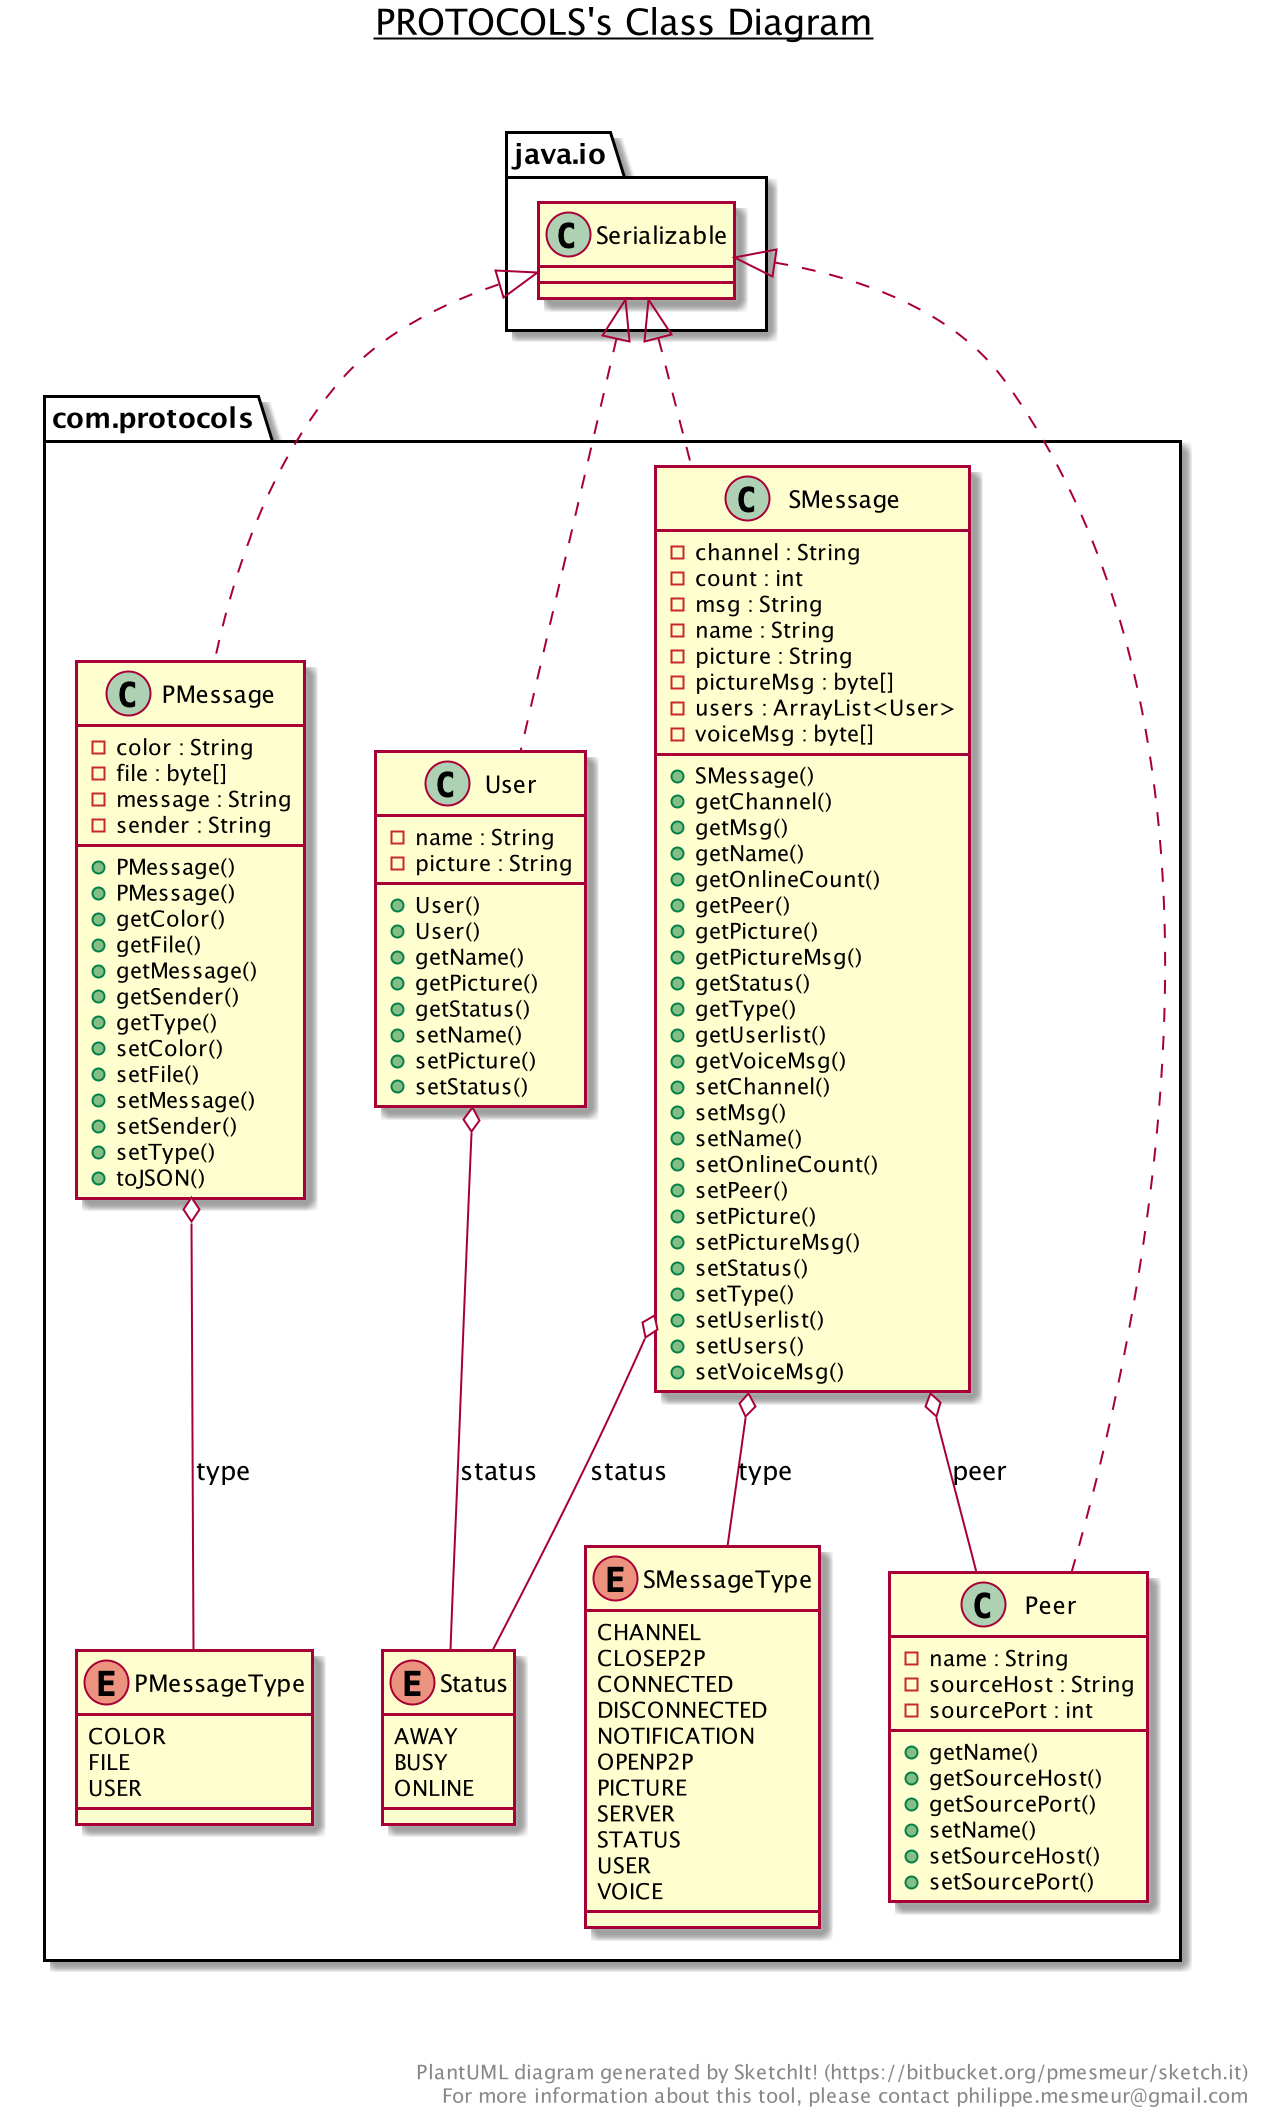
\includegraphics[height=13cm]{protocols}
	\caption{Mô hình định nghĩa giao thức giao tiếp trong ứng dụng}
\end{figure}

Ứng dụng sử dụng 2 giao thức: giao thức sử dụng trong giao tiếp giữa client-server (dựa trên giao thức TCP) và giao thức sử dụng trong giao tiếp giữa client-client (dựa trên giao thức UDP).


\subsection{Giao thức giao tiếp client-server}
Client giao tiếp với Server để thức hiện các chức năng: thông báo đăng nhập/đăng xuất; thay đổi trạng thái hoạt động; gửi công khai/riêng tư tin nhắn, ảnh, âm thanh sử dụng giao thức TCP; thiết lập kết nối UDP trực tiếp với client khác.

Giao thức gồm các trường thông tin chính sau:
\begin{enumerate}
	\item {\bf name: String.} Thông tin về client (tên đăng nhập).
	\item {\bf type: SMessageType.} Chức năng yêu cầu server xử lý, gồm có: 
	\begin{itemize}
		\item[-] DISCONNECTED
		\item[-] CONNECTED 
		\item[-] STATUS
		\item[-] USER
		\item[-] SERVER
		\item[-] NOTIFICATION
		\item[-] VOICE
		\item[-] CHANNEL
		\item[-] PICTURE.
		\item[-] OPENP2P
		\item[-] CLOSEP2P
	\end{itemize}
	\item {\bf channel: String.} Thông tin về {\bf kênh} đang giao tiếp, gồm: {\bf \#Community} - tin nhắn gửi công khai đến toàn bộ người dùng, {\bf Personal} - tin nhắn gửi riêng đến người dùng xác định (toàn bộ dựa trên giao thức TCP, tức là client - server - client).
	\item {\bf count: Integer.} Số lượng người dùng.
	\item {\bf status: Status.} Trạng thái hoạt động của người dùng: ONLINE, AWAY, BUSY.
	\item {\bf users: User.} Danh sách người dùng.
	\item {\bf picture: String.} Đường dẫn đến ảnh người dùng.
	\item {\bf msg: String.} Nội dung tin nhắn văn bản.
	\item {\bf pictureMsg: byte[].} Nội dung của ảnh được mã hoá theo chuẩn Base64.
	\item {\bf voiceMsg: byte[].} Nội dung của âm thanh được mã hoá.
\end{enumerate}

 

\subsection{Giao thức giao tiếp client-client}

Giao thức sử dụng trong giao tiếp trực tiếp giữa 2 client với nhau (dựa trên UDP):

\begin{enumerate}
	\item {\bf sender: String.} Thông tin người gửi (tên).
	\item {\bf message: String.} Nội dung tin nhắn văn bản.
	\item {\bf type: PMessageType.} Chức năng yêu cầu, gồm: USER, FILE, COLOR.
	\item {\bf file: byte[].} Nội dung file được mã hoá theo chuẩn Base64.
	\item {\bf color: String.} Mã hex của màu cuộc trò chuyện.
\end{enumerate}

\section{Miêu tả chi tiết hiện thực chức năng}

\subsection{Chức năng trên client-server}
Server có thể phục vụ cùng lúc nhiều yêu cầu từ client, tạo nhiều thread, trong đó, 1 thread {\bf master} chuyên ghi nhận các socket kết nối đến server và nhiều thread (các {\bf handle}) xử lý các yêu cầu chức năng tương ứng với từng client trong quá trình giao tiếp. 

Các chức năng yêu cầu được xác định dựa vào trường thông tin {\bf type.} của mỗi message gửi từ client.

Message sẽ được truyền theo đường đi client-server-clients.
\subsubsection{Đăng nhập/đăng xuất ứng dụng.}
Server cho phép người dùng sử dụng một tên đăng nhập để đăng ký vào Lobby của ứng dụng. Tên đăng nhập này là duy nhất. 

Server sẽ lưu trữ các người dùng thông qua HashMap từ {\tt username} đến {user} tương ứng. Nhờ đó trên mỗi {\bf handle} chỉ cần lưu một trường thông tin là {\tt username} vẫn có thể truy xuất thông tin về người dùng cũng như kiểm tra tên đăng nhập đã tồn tại hay chưa.

Khi người dùng đăng nhập/đăng xuất, một message có {\bf kiểu} là {\it CONNECTED/DISCONNECTED} sẽ được gửi từ client đến server, server sẽ ghi nhận và thông báo đến toàn bộ \#Community (cùng kiểu với message nhận từ client) để cập nhận danh sách trạng thái trên khung hiện thị của mỗi client.

\subsubsection{Thay đổi trạng thái hoạt động}
Thông tin trạng thái hoạt động của người dùng được lưu tại trường thông tin {\bf status.} trên mỗi message mỗi khi client gửi yêu cầu thay đổi trạng thái đến server.

Server sẽ ghi nhận và gửi đến toàn \# Community (kể cả client gửi request) để cập nhật trạng thái hoạt động hiện thị trên khung lobby của mỗi client.


\subsubsection{Gửi công khai tin nhắn văn bản/ảnh/âm thanh}
Nội dung tin nhắn văn bản hoặc ảnh hoặc âm thanh được mã hoá và lưu trữ tại các trường {\bf msg.} hoặc {\bf pictureMsg.} hoặc {\bf voiceMsg.}.

Server ghi nhận và gửi response đến toàn bộ \#Community.

\subsubsection{Gửi riêng tư tin nhắn văn bản hoặc ảnh hoặc âm thanh.}
Người dùng có thể tuỳ ý thay đổi kênh giao tiếp bằng cách trỏ đến các kênh xác định có trên khung chat. Một message mang theo thông tin kênh lưu trữ tại trường {\bf channel.} được gửi đến Server (một {\bf handle}). Trên server cũng sẽ có một trường lưu trữ thông tin về kênh giao tiếp hiện tại đang phục vụ. 

Việc cập nhật kênh giao tiếp sẽ được thức hiện trước khi việc gửi tin nhắn riêng tư được thức hiện.  Điểm khác biệt khi gửi tin nhắn riêng tư (so với gửi công khai) là chỉ người nhận (và người gửi) nhận được tin nhắn. Đường đi của message sẽ đi từ người gửi - server - (người nhận - người gửi).

\subsubsection{Yêu cầu mở/tắt giao tiếp UDP giữa 2 client}
 Khi người dùng muốn thiết lập một giao tiếp UDP với người dùng khác. Một message có {\bf type.} là {\bf SMessageType.OPENP2P} kèm theo thông tin về người dùng đầu bên kia (tên đăng nhập) được lưu trữ tại trường {\bf peer.} được gửi theo đường {\it client 1 - server - client 2}. Client 2 nhận message sẽ gửi lại một message tương ứng đến client 1. và giao tiếp UDP được thiết lập. 
Trường này lưu trữ ba thông tin: 
 	\begin{itemize}
		\item[-] {\bf name.} Tên đăng nhập của người dùng bên kia.
		\item[-] {\bf host.} Địa chỉ IP của người dùng bên này.
		\item[-] {\bf port.} Port gửi của người dùng bên này.
	\end{itemize} 
	
 
\subsection{Các chức năng trên client-client}

Khác với mô hình client-server, mô hình client-client sử dụng giao thức UDP. Trên mỗi client sẽ có hai thanh phần, một cho xử lý thông tin nhận vào {\bf Receiver}, một xử lý thông tin gửi đi {\bf Sender}.

Tuỳ vào từng chức năng mà người dùng thực hiện, {\bf sender} sẽ đóng gói thông tin trong protocol-message và gửi đến trực tiếp người dùng đang giao tiếp bên đầu kia. {\bf Receiver} nhận gói tin và trích các thông tin trên đó để ghi nhận và xử lý phù hợp. Để rõ hơn ta sẽ đi vào từng chức năng cụ thể:

\subsubsection{Gửi tin nhắn văn bản}
{\bf Sender} sẽ đóng gọi protocol-message gồm các 5 trường thông tin (như mô tả ở trên):
\begin{itemize}
	\item {\bf sender.} lưu thông tin về người gửi.
	\item {\bf type.} gắn thông tin PMessageType.USER - giao tiếp bằng tin nhắn văn bản.
	\item {\bf message.} gắn nội dụng tin nhắn.
	\item {\bf file.} và {\bf color.} được để trống (null).
\end{itemize}

{\bf Receiver} sẽ nhận protocol-message sau đó ghi nhận chức năng bằng trường thông tin {\bf type.}

\subsubsection{Gửi file}

{\bf Sender} sẽ mã hoá nội dung file theo chuẩn Base64 và lưu trữ nó trong trường thông tin {\bf file.} của protocol-message.

Kèm theo tên file được lưu vào trường thông tin {\bf message.} Lúc này {\bf type.} sẽ giữ giá trị {\tt PMessageType.FILE}.

{\bf Receiver} nhận message từ {\bf sender} bên gửi, ghi nhận thông tin tại trường {\bf type.} để có cách phù hợp xử lý gói tin đến.

\subsubsection{Đổi màu cuộc trò chuyện}

Người dùng sẽ chọn màu hiển thị khi mở bảng màu trên GUI, {\bf sender} ghi nhận màu dưới dạng HEX và lưu thông tin tại trường {\bf color.} Lúc này, {\bf type.} sẽ giữ giá trị {\tt PMessageType.COLOR}.
\newpage

\section{Thiết kế chi tiết}
\subsection{Kiến trúc tổng quát}

\begin{figure}[h!]
	\centering
	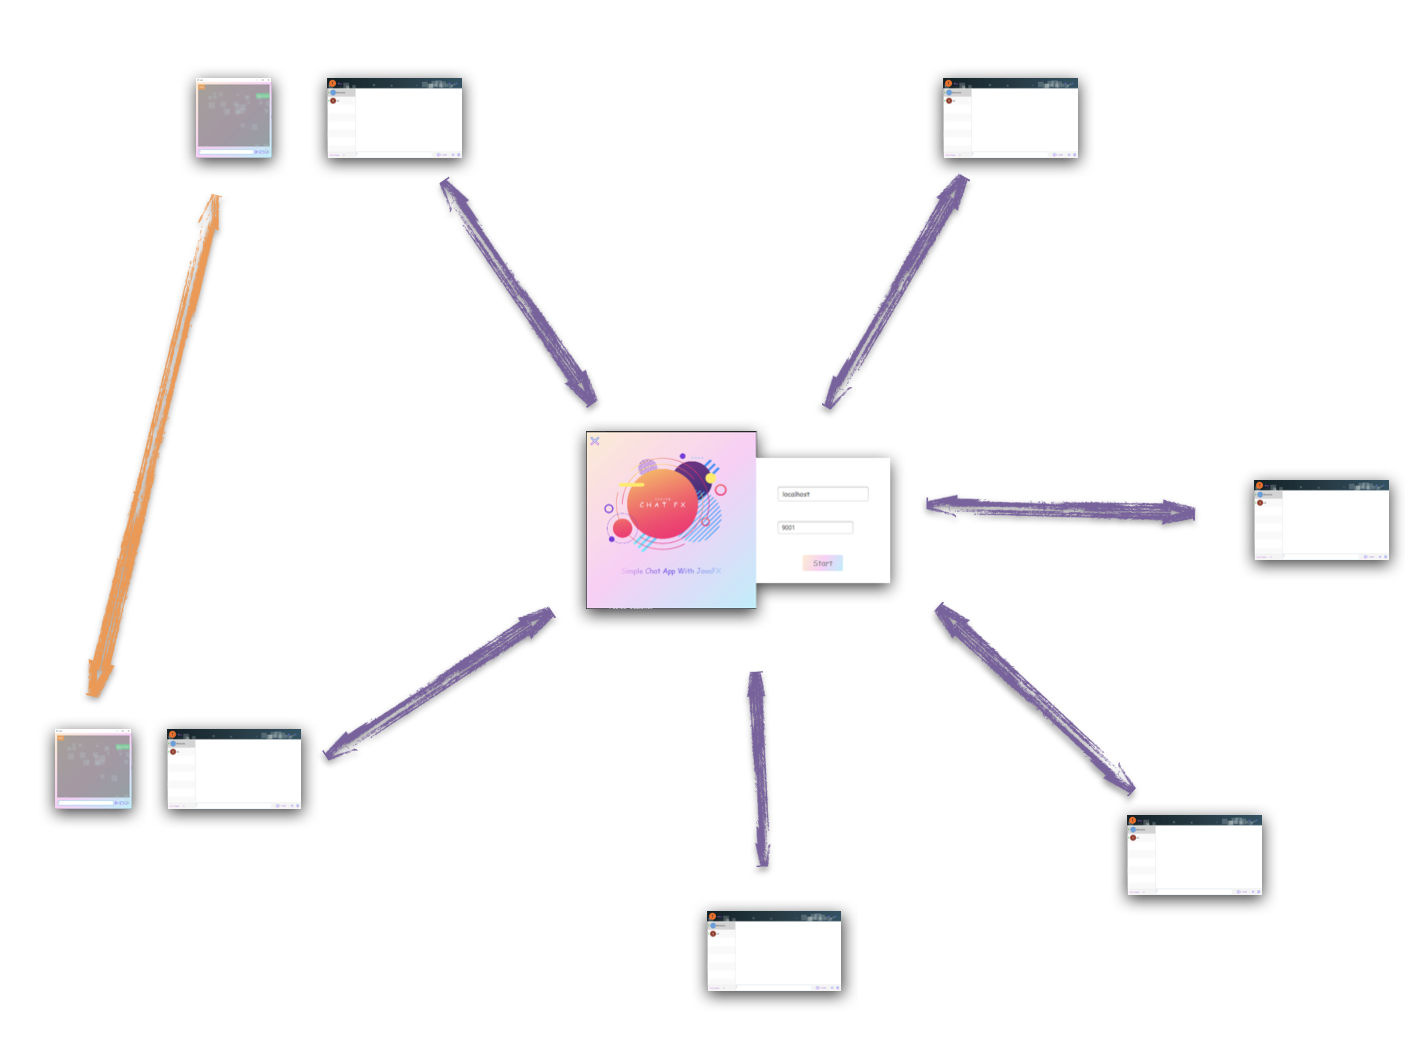
\includegraphics[width=11cm]{architecture}
	\caption{Kiến trúc tổng quát}
\end{figure}

Như đã trình bày ở phần trên, mỗi client sẽ đăng nhập và chuyển đến phòng chat chung. Nơi hiển thị tin nhắn đến cũng như thực hiện các chức năng cửa ứng dụng.

\newpage
\subsection{Lược đồ lớp}

Các package chính trong ứng dụng:
\begin{itemize}
	\item {\bf com.server} - Gồm các class để hiển thực SocketServer cùng GUI, trong đó class {\bf Server.java} hiện thực để xử lý các yêu cầu chức năng chính.
	\begin{figure}[h!]
		\centering
		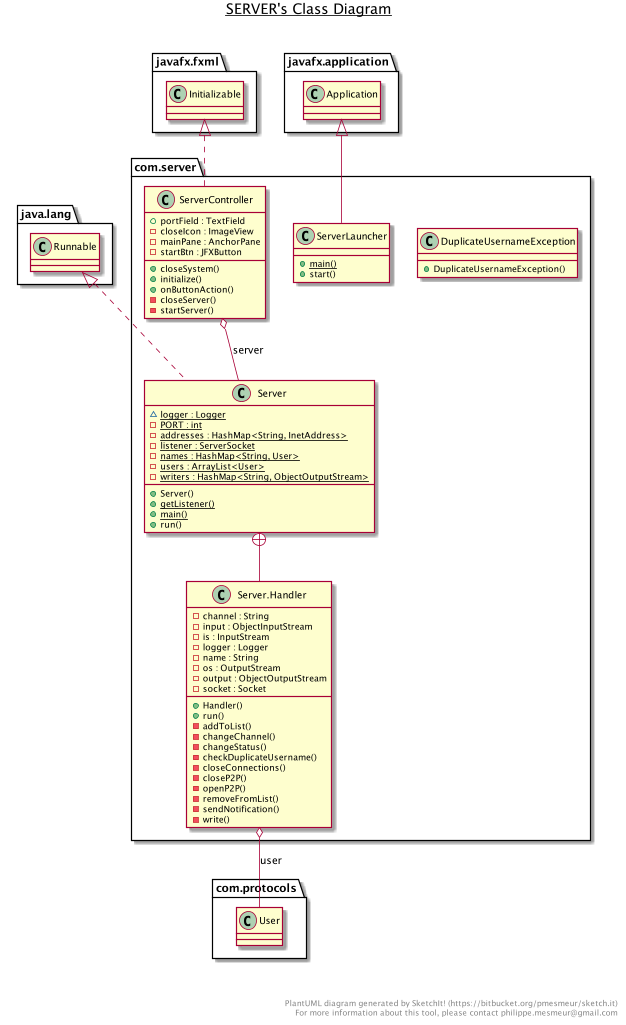
\includegraphics[width=11cm]{plantuml-server}
		\caption{Lược đồ lớp package com.server}
	\end{figure}
	\newpage
	\item {\bf com.protocols} - Gồm các class định nghĩa các giao thức sử dụng trong ứng dụng, như: {\bf SMessage} - giao thức giao tiếp giữa client-server; {\bf PMessage} - giao thức giao tiếp client-client.
	\begin{figure}[h!]
		\centering
		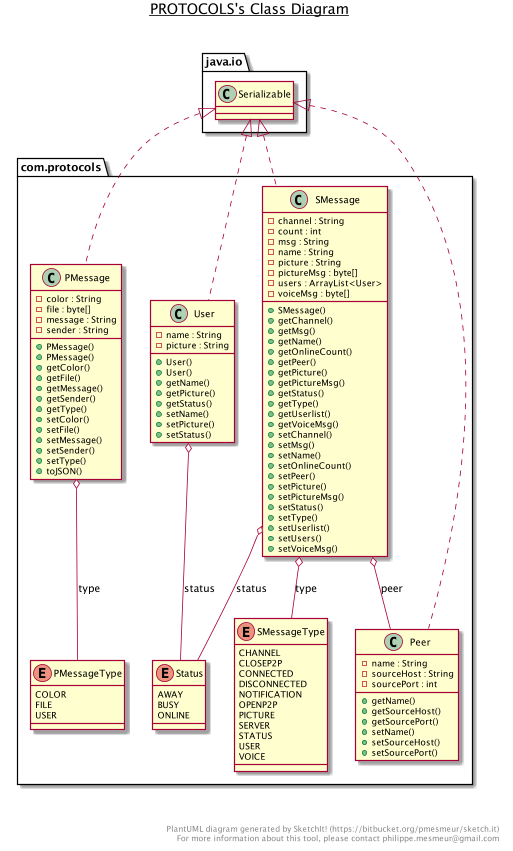
\includegraphics[width=11cm]{plantuml-protocols}
		\caption{Lược đồ lớp package com.protocols}
	\end{figure}
	\newpage
	\item {\bf com.lobby} - Gồm các class hiện thực phần front-end, cung cấp cách thức giao tiếp giữa người dùng và server.
	\begin{figure}[h!]
		\centering
		\begin{tabular}{c c}
 	 		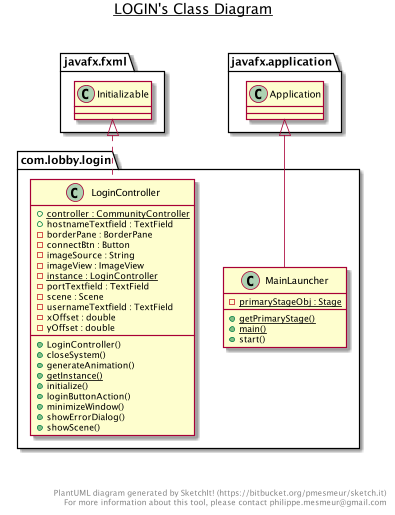
\includegraphics[width=7cm]{plantuml-login} &
 	 		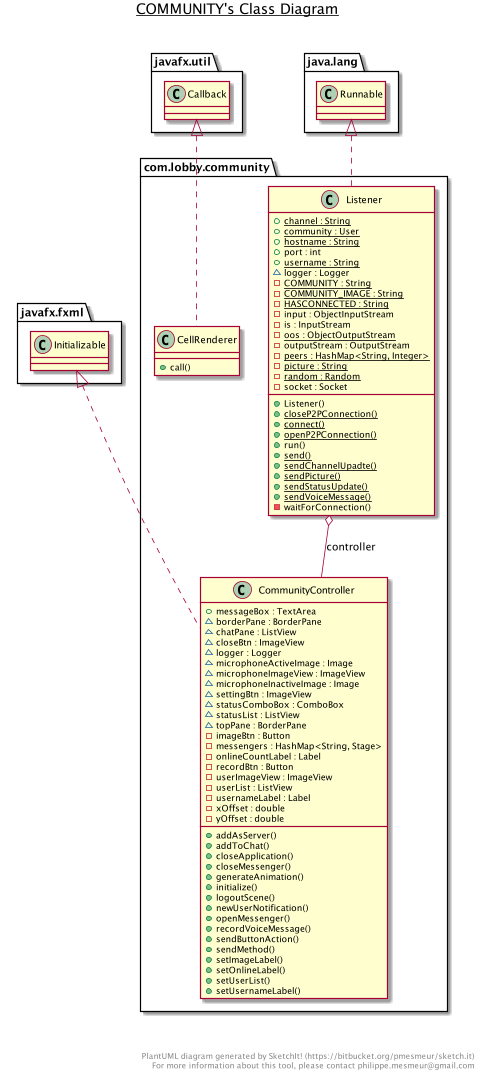
\includegraphics[width=7cm]{plantuml-community}
		\end{tabular}
		\caption{Lược đồ các lớp trong package com.lobby}
	\end{figure}
	\newpage
	\item {\bf com.messenger} - Gồm các class hiện thực giao tiếp trực tiếp giữa client-client. 
	\begin{figure}[h!]
		\centering
		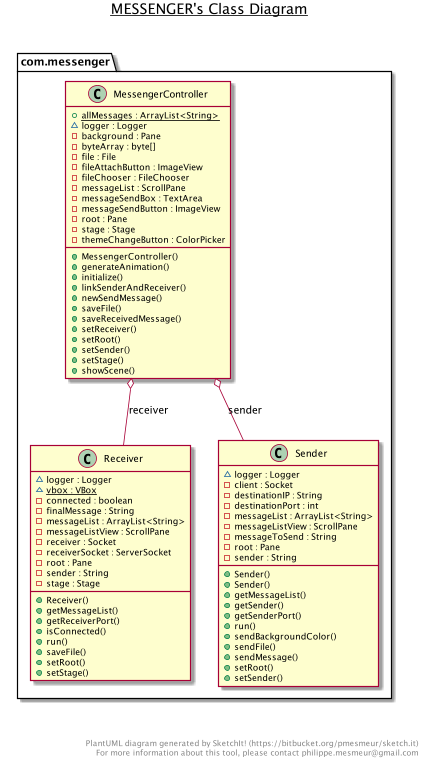
\includegraphics[width=9cm]{plantuml-messenger}
		\caption{Lược đồ lớp package com.messenger}
	\end{figure}
\end{itemize}

\newpage
\section{Đánh giá kết quả hiện thực}
	  \subsection{Khởi động server}
	Cách 1: sử dụng server CLI:
	\begin{itemize}
		\item Chạy class com.server.Server.
		\newline
		\begin{figure}[h!]
			\centering
			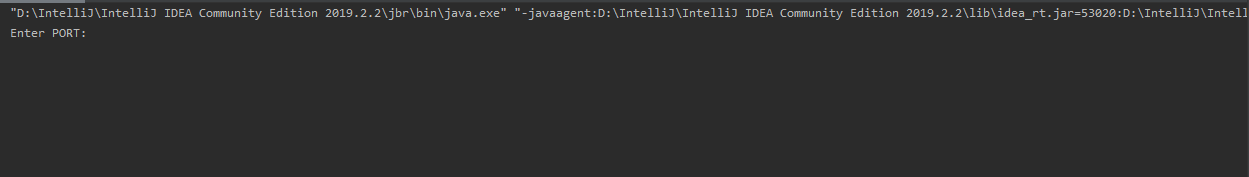
\includegraphics[width=\linewidth]{server_CLI.PNG}
			\caption{Server CLI}
			\label{fig:my_label}
		\end{figure}
		\item Nhập tên port vào. VD: 9001.
	\end{itemize}
	Cách 2: sử dụng server UI:
	\begin{itemize}
		\item Chạy class com.server.ServerController.
		\newline
		\begin{figure}[h!]
			\centering
			\begin{tabular}{c c}
				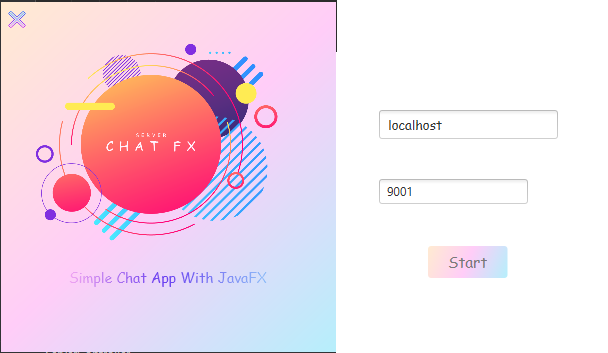
\includegraphics[width=7cm]{server_Launcher.PNG} &
			
				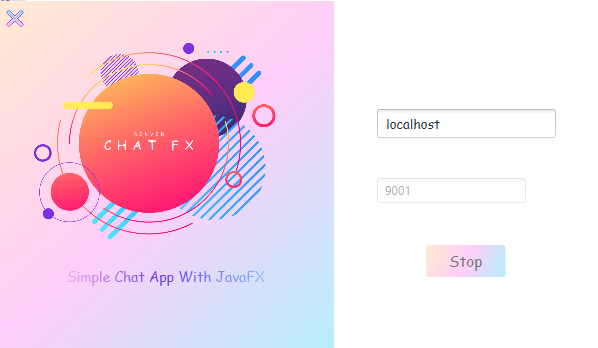
\includegraphics[width=7cm]{stop-server.PNG}
			\end{tabular}
			\caption{Server UI}
			\label{fig:my_label}
		\end{figure}
		\item Nhập đường dẫn vào server ở ô localhost. Nhập port vào ô dưới rồi bấm nút Start để khởi động server.
		\item Để tắt server nhấn nút stop
	\end{itemize}
	\subsection{Đăng nhập}
	Chạy class com.client.login.Mainlauncher.

		
	\begin{itemize}
		\item Nhập tên người dùng vào ô username.
		\item Nhập đường dẫn tới server vào hostname.
		\item Nhập port kết nối.
	\end{itemize}
	\newpage
	\begin{figure}[h!]
		\centering
		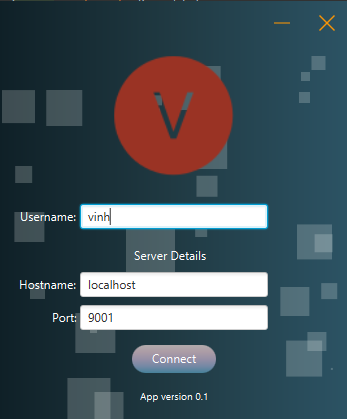
\includegraphics[width=7cm]{LogIn.PNG}
		\caption{Màn hình Login}
		\label{fig:my_label}
	\end{figure}

	Giao diện sau khi đăng nhập thành công vào server.
	\begin{figure}[h!]
		\centering
		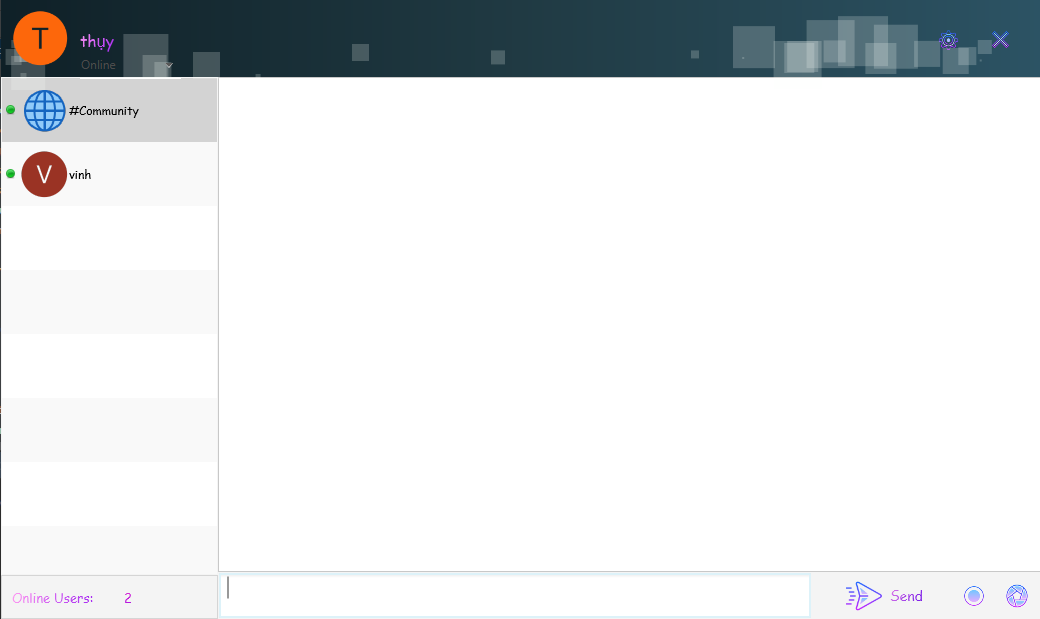
\includegraphics[width=13cm]{interface.PNG}
		\caption{Main Interface}
		\label{fig:my_label}
	\end{figure}
	\subsection{Gửi tin nhắn}
	\subsubsection{Gửi tin nhắn vào phòng chat chung}
	\begin{itemize}
		\item Nhấn chọn kênh chat community
		\newpage
		\item Nhập tin nhắn từ bàn phím vào ô chat dưới cùng
		\begin{figure}[h!]
			\centering
			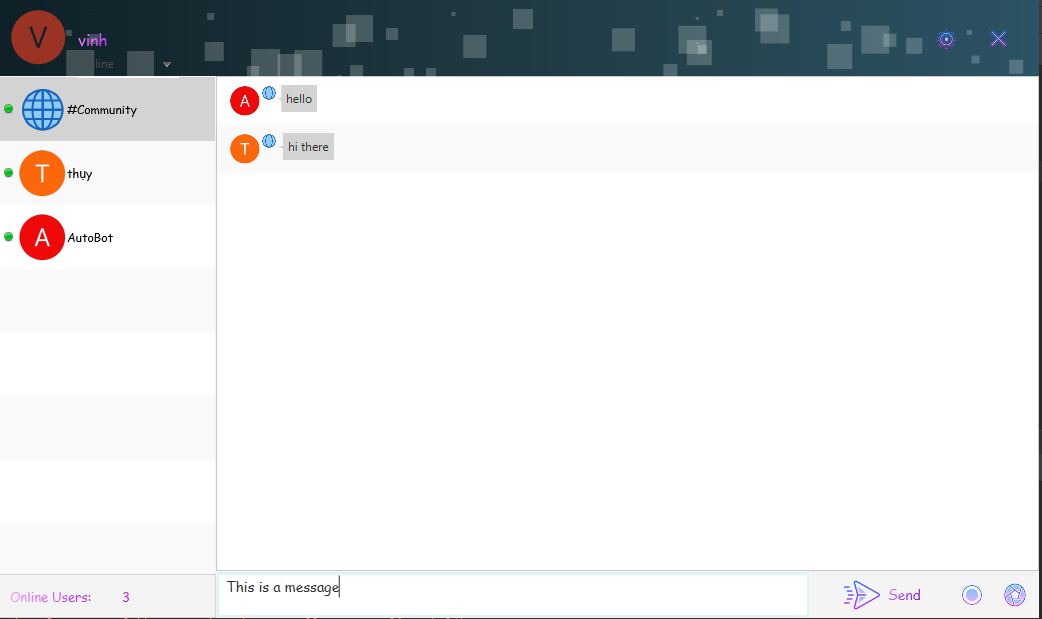
\includegraphics[width=13cm]{enter-message.PNG}
			\caption{Send public message}
			\label{fig:my_label}
		\end{figure}
		\item Bấm enter hoặc nhấn nút send cạnh ô chat sẽ được kết quả như hình
		\begin{figure}[h!]
			\centering
			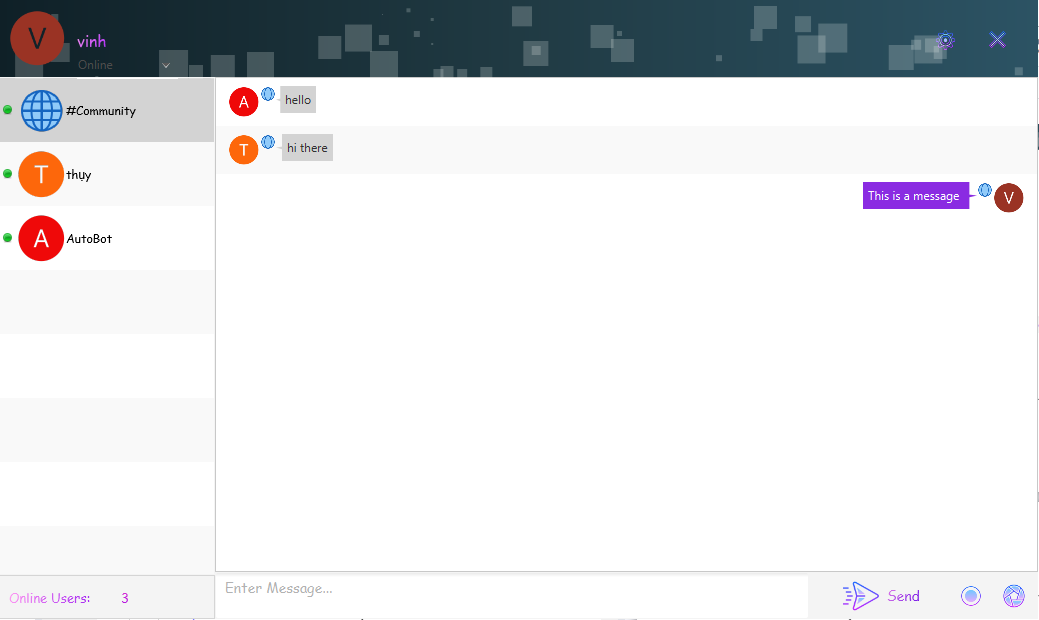
\includegraphics[width=13cm]{message-sent.PNG}
			\caption{Message sent in community channel}
			\label{fig:my_label}
		\end{figure}
		\newpage
		\item Để gửi tin nhắn thoại nhấn vào nút thu âm bên phải nút send và bắt đầu nói.
		\begin{figure}[h!]
			\centering
			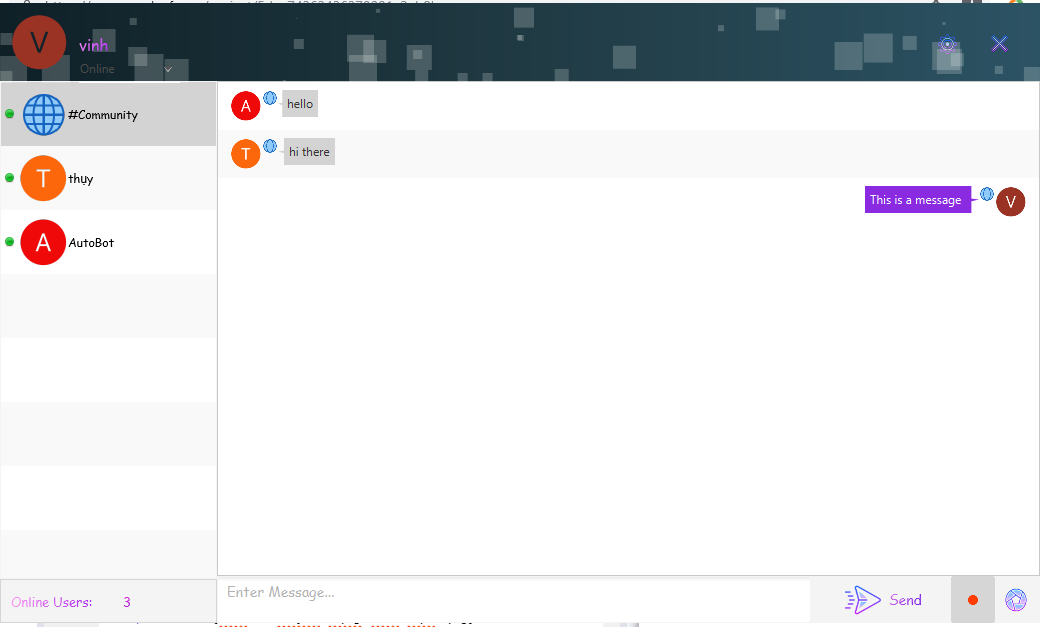
\includegraphics[width=13cm]{send-voice-message.PNG}
			\caption{Send voice message}
			\label{fig:my_label}
		\end{figure}
		\item Nhấn vào nút thu âm 1 lần nữa để gửi đi. Kết quả như hình sau.
		\begin{figure}[h!]
			\centering
			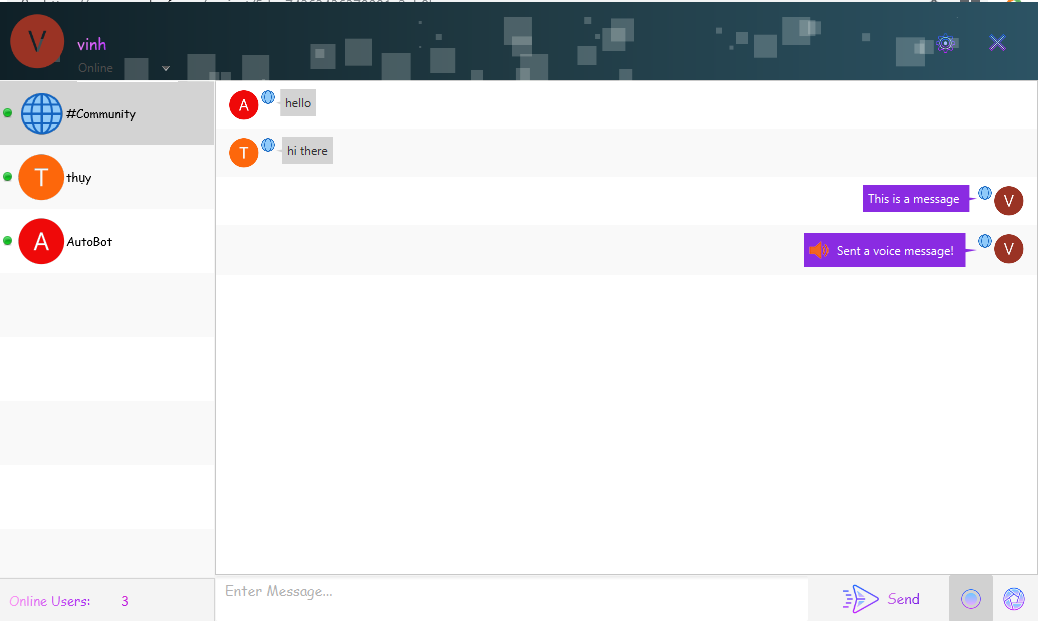
\includegraphics[width=13cm]{voice-message.PNG}
			\caption{Voice message sent}
			\label{fig:my_label}
		\end{figure}
		\newpage
		\item Để gửi file nhấn vào nút duyệt file bên phải nút thu âm để mở hộp thoại chọn thư mục.
		\begin{figure}[h!]
			\centering
			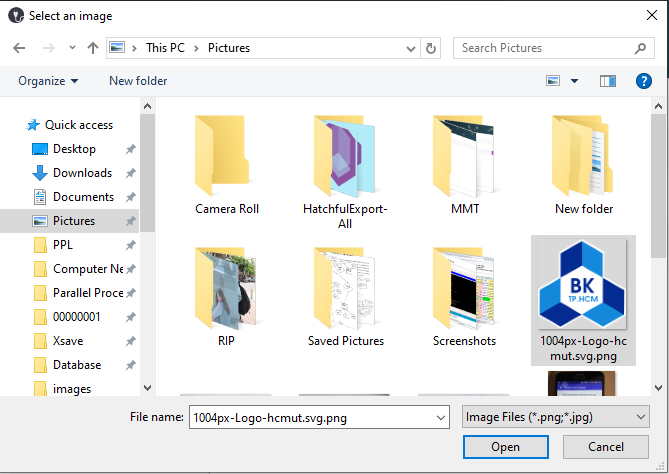
\includegraphics[width=13cm]{send-file.PNG}
			\caption{Browse file}
			\label{fig:my_label}
		\end{figure}
		\item Nhấn vào file cần chọn. Kết quả như hình sau.
		\begin{figure}[h!]
			\centering
			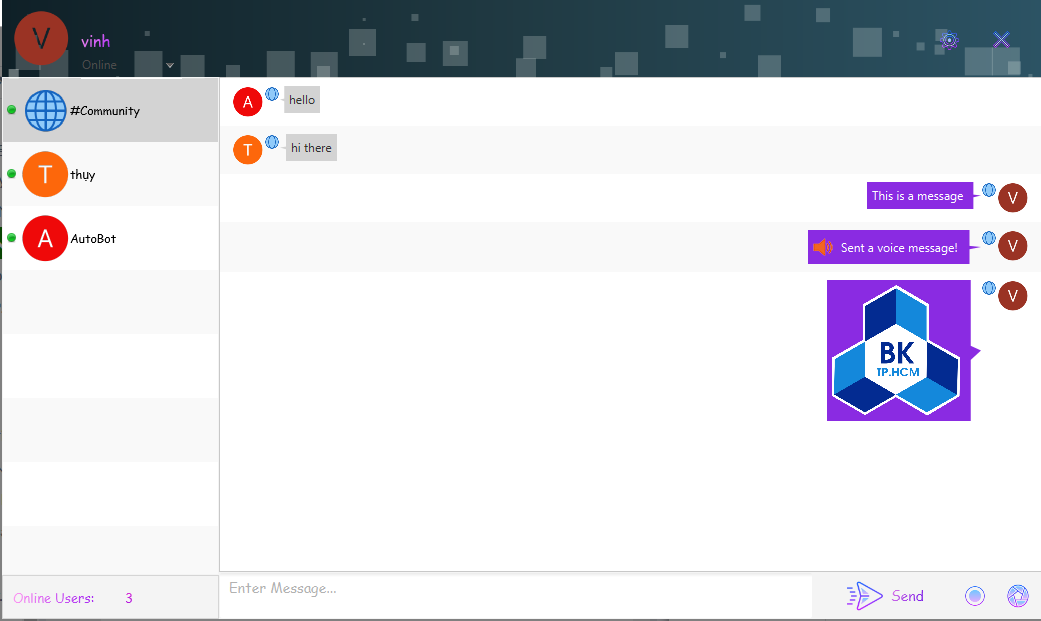
\includegraphics[width=13cm]{file-sent.PNG}
			\caption{File sent}
			\label{fig:my_label}
		\end{figure}
	\end{itemize}
	\newpage
	\subsubsection{Gửi tin nhắn riêng cho user khác}
	\begin{itemize}
		\item Nhấp chọn user để gửi tin nhắn đến.
		\item Cửa sổ chat mới hiện ra.     
		\begin{figure}[h!]
			\centering
			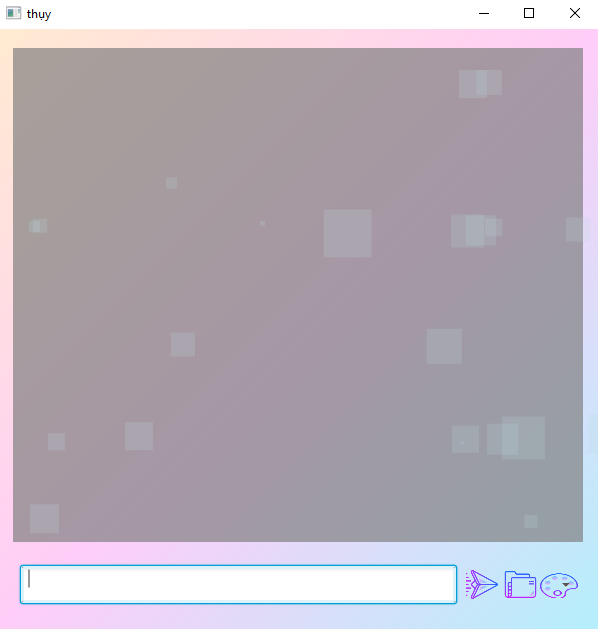
\includegraphics[width=9cm]{start-chat-private.PNG}
			\caption{Send private message}
			\label{fig:my_label}
		\end{figure}
		\item Nhập tin nhắn từ bàn phím vào ô chat dưới cùng.
		\begin{figure}[h!]
			\centering
			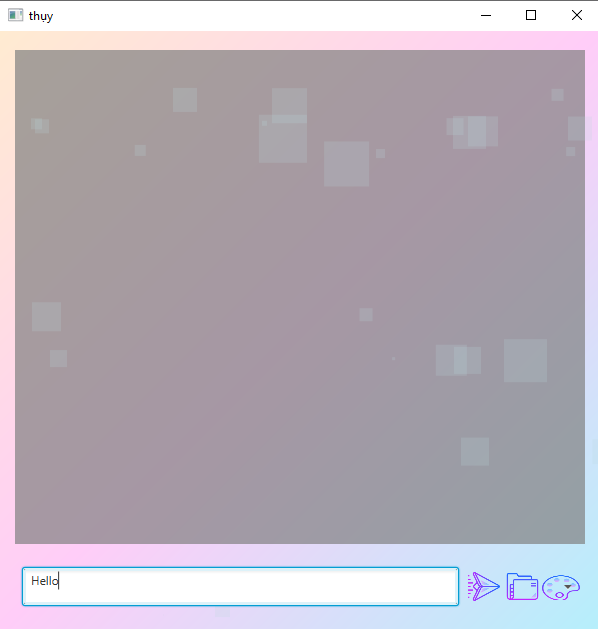
\includegraphics[width=8cm]{enter-message-private.PNG}
			\caption{Enter private message}
			\label{fig:my_label}
		\end{figure}
		\item Nhấn nút send ở bên cạnh ô chat hoặc nhấn phím enter để gửi tin.
		\begin{figure}[h!]
			\centering
			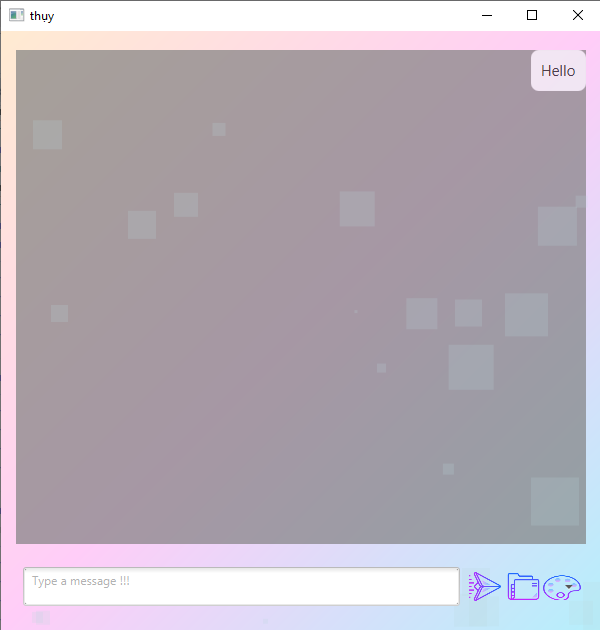
\includegraphics[width=8cm]{message-sent-private.PNG}
			\caption{Private message sent}
			\label{fig:my_label}
		\end{figure}
		\newpage
		\item Để gửi tệp tin nhấn nút hình tệp tin cạnh nút send để mở hộp thoại chọn thư mục.
		\begin{figure}[h!]
			\centering
			\begin{tabular}{c c}
			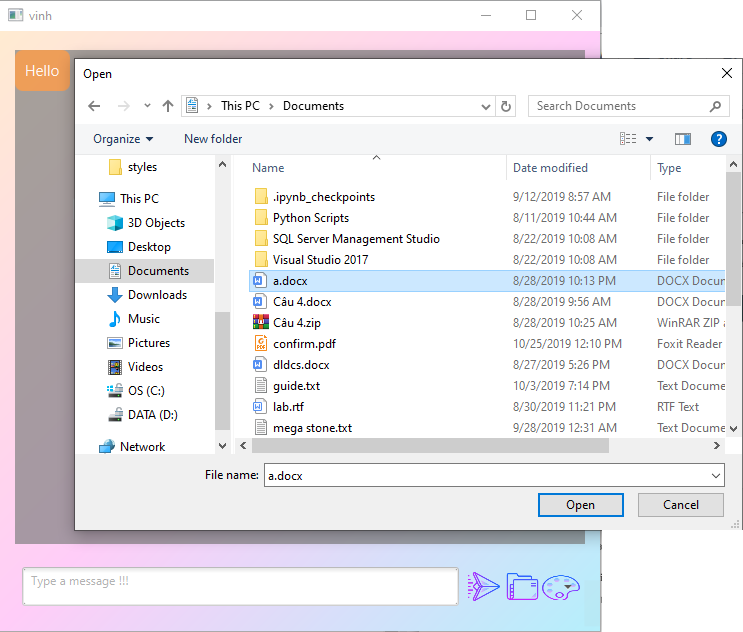
\includegraphics[width=8cm]{browse-directory-private.PNG} &
			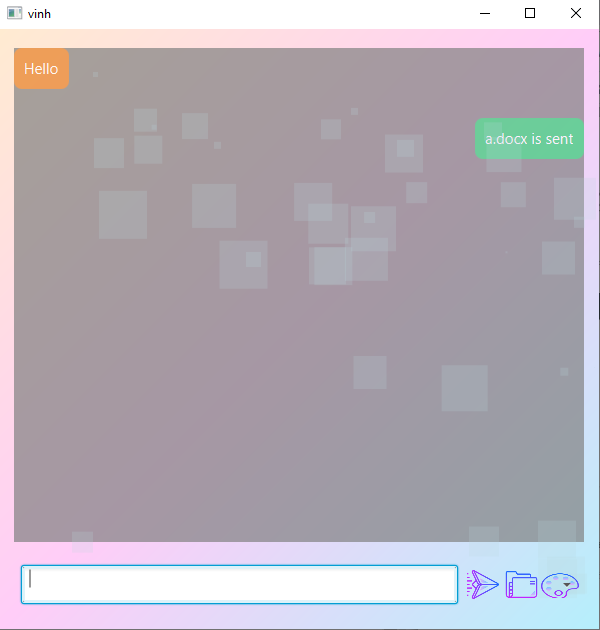
\includegraphics[width=7cm]{private-file-sent.PNG}
			\end{tabular}
			\caption{Browse directory private}
			\label{fig:my_label}
		\end{figure}
		\item Nhấn open để gửi
		\newpage
		\item Để đồi màu bóng chat nhấn chọn nút bảng màu nằm bên phải nút chọn file và chọn màu.
		\begin{figure}[h!]
			\centering
			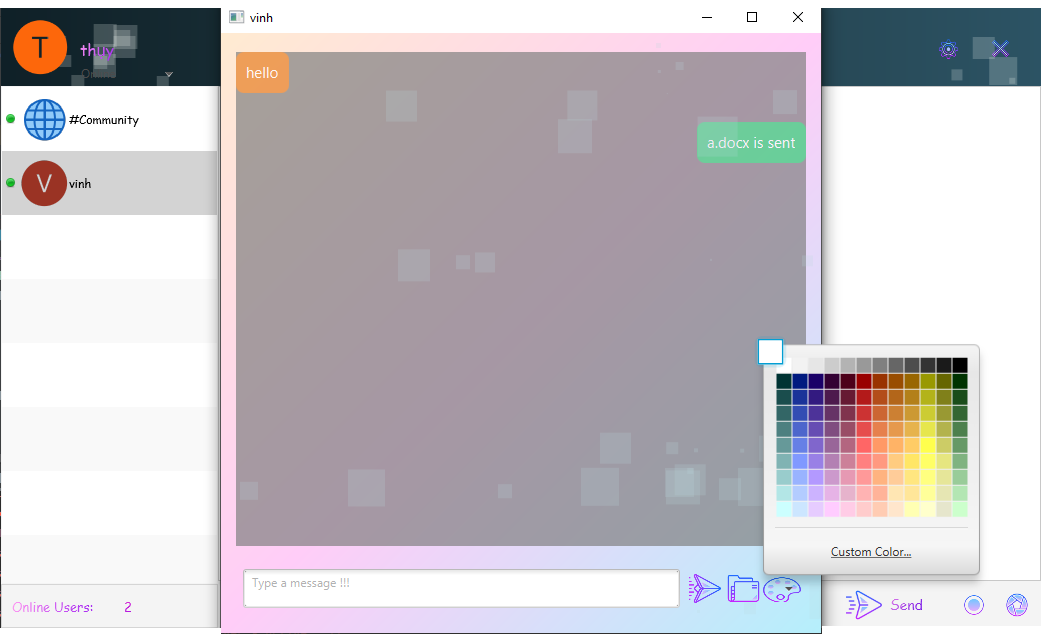
\includegraphics[width=8cm]{browse-color.png}
			\caption{Change chat bubble's color}
			\label{fig:my_label}
		\end{figure}
		\item Kết quả như hình sau.
		\begin{figure}[h!]
			\centering
			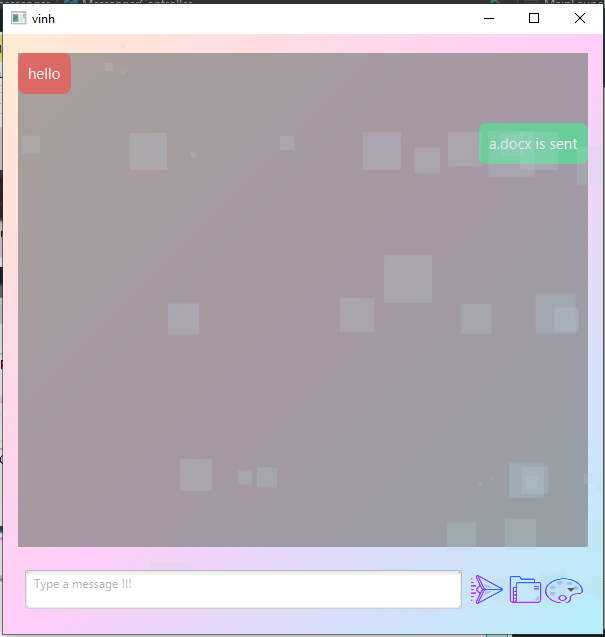
\includegraphics[width=8cm]{color-changed.PNG}
			\caption{Chat bubble's color changed}
			\label{fig:my_label}
		\end{figure}
	\end{itemize}
	\newpage
	\subsection{Chuyển trạng thái hoạt động}
	Nhấn vào dấu mũi tên ở dưới username góc trên cùng bên trái để mở bảng chuyển trạng thái.
	\begin{figure}[h!]
		\centering
		\begin{tabular}{c c}
		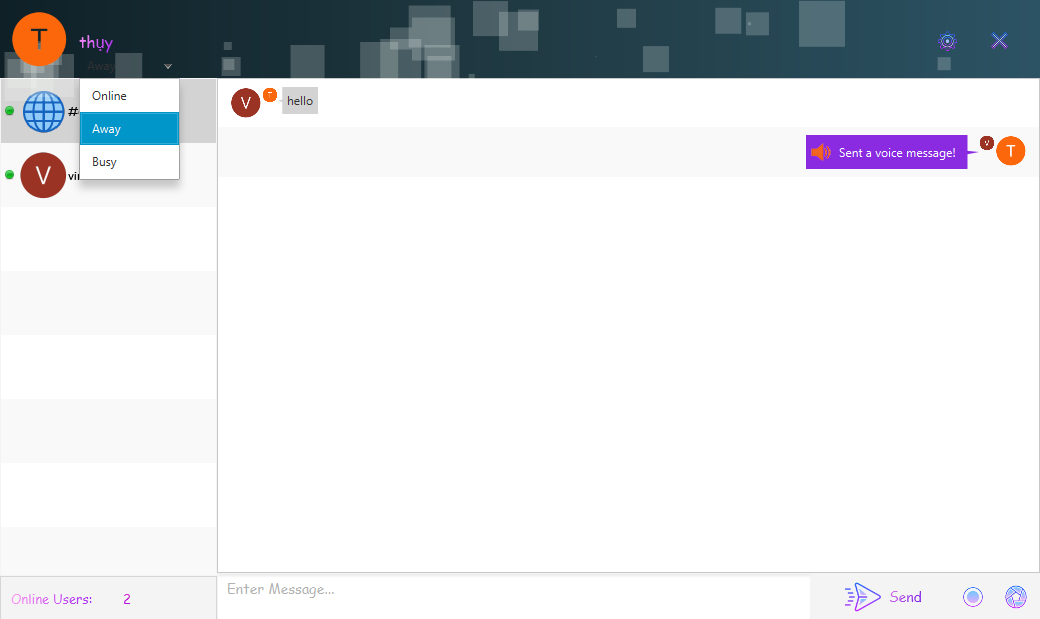
\includegraphics[width=11cm]{state-change.png} &
		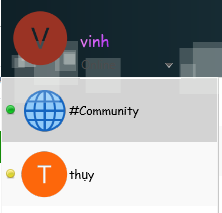
\includegraphics[width=3cm]{state-changed.PNG}
		\end{tabular}
		\caption{Change state}
		\label{fig:my_label}
	\end{figure}
	Sau khi đổi trạng thái, dấu tích ở bên cạnh username sẽ đổi màu đối với các user khác.

\newpage
\begin{thebibliography}{9}
\bibitem{gpcoder.com} 
GPCoder
\textit{Xây dựng ứng dụng Client-Server với Socket trong Java}. \\
last visited Oct 28th, 2019.
 
\bibitem{keeptoo} 
KeepToo
\textit{JavaFX UI design youtube channel }.\\
Last seen Oct 25th, 2019.
 
\bibitem{oracle} 
\texttt{https://docs.oracle.com/javase/tutorial/}. \\
Last visited Oct 28th, 2019.
\end{thebibliography}

\newpage
\appendix
\section{Hướng dẫn sử dụng}

Thư mục {\it app/} (như hình dưới) chứa các artifacts (file .jar) để mở ứng dụng. 

\begin{figure}[h!]
	\centering
	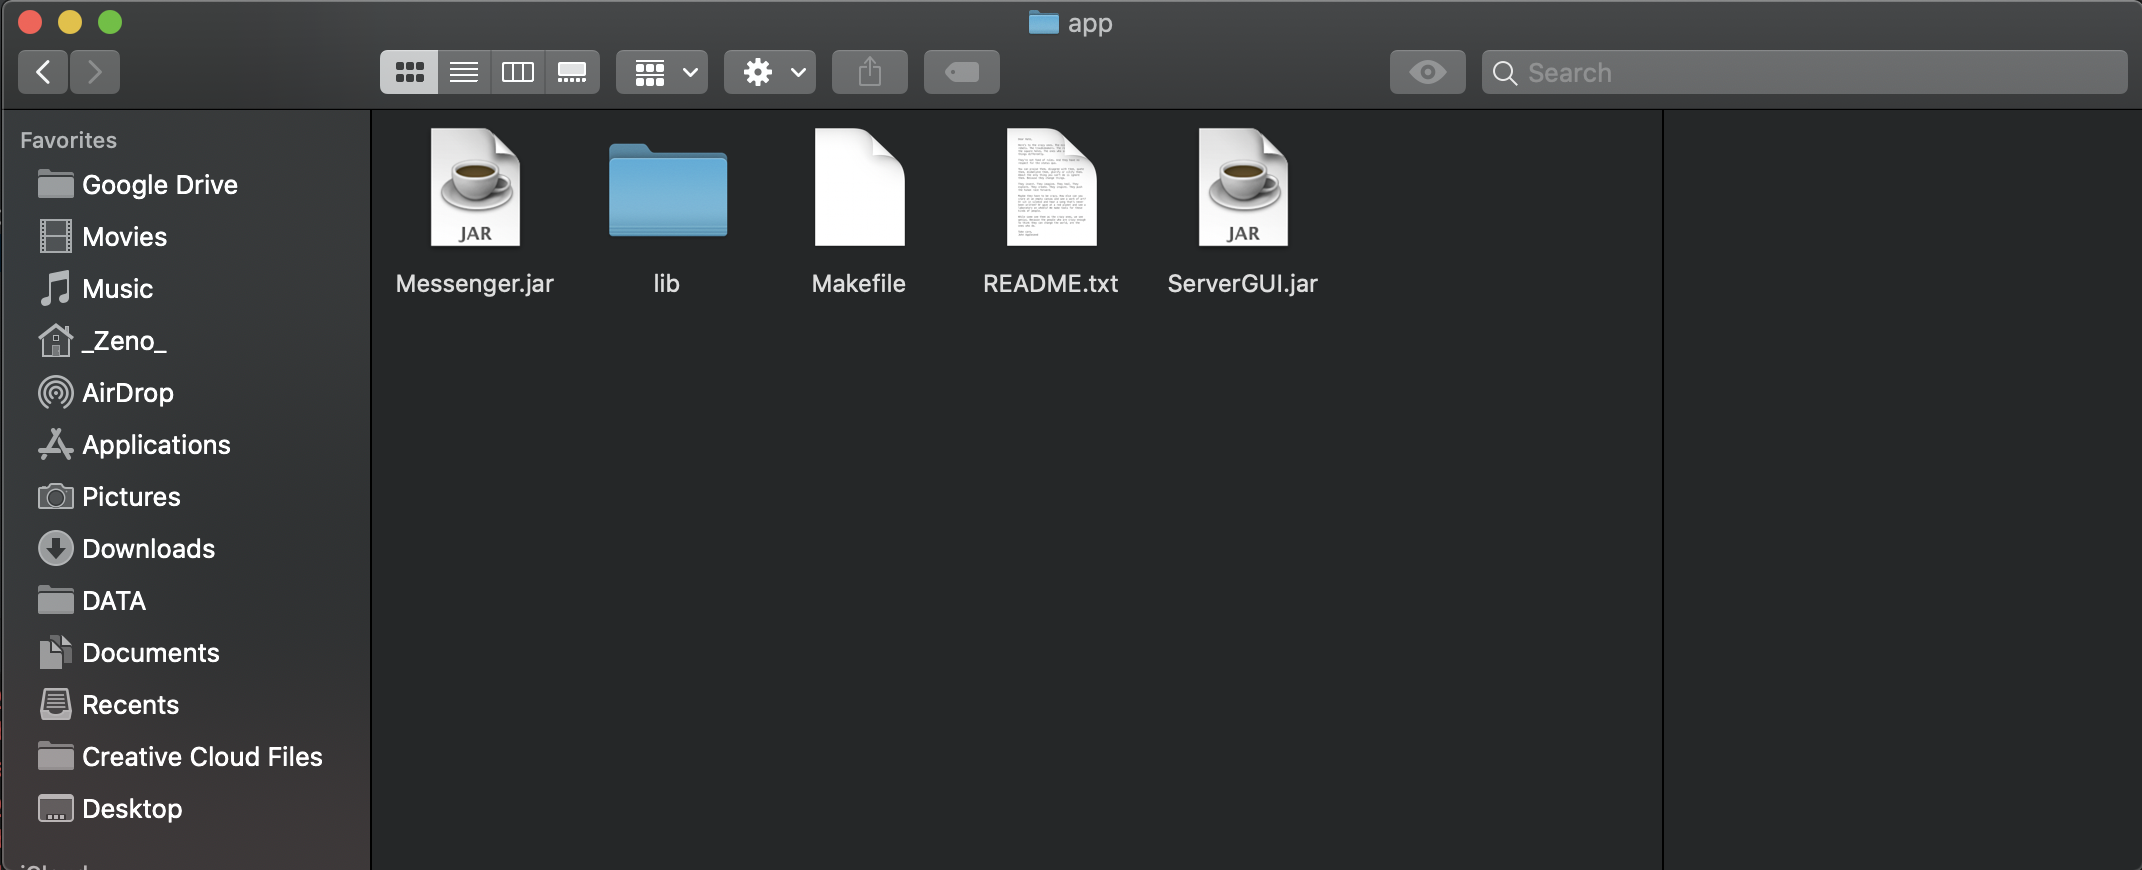
\includegraphics[width=11cm]{app-folder}
	\caption{Thư mục app chưa artifacts để mở ứng dụng}
\end{figure}

Mở terminal trỏ đến thư mục hiện tại và chạy hai dòng lệnh để khởi dộng ứng dụng {\tt make Client} 

\begin{figure}[h!]
	\centering
	\begin{tabular}{c c}
	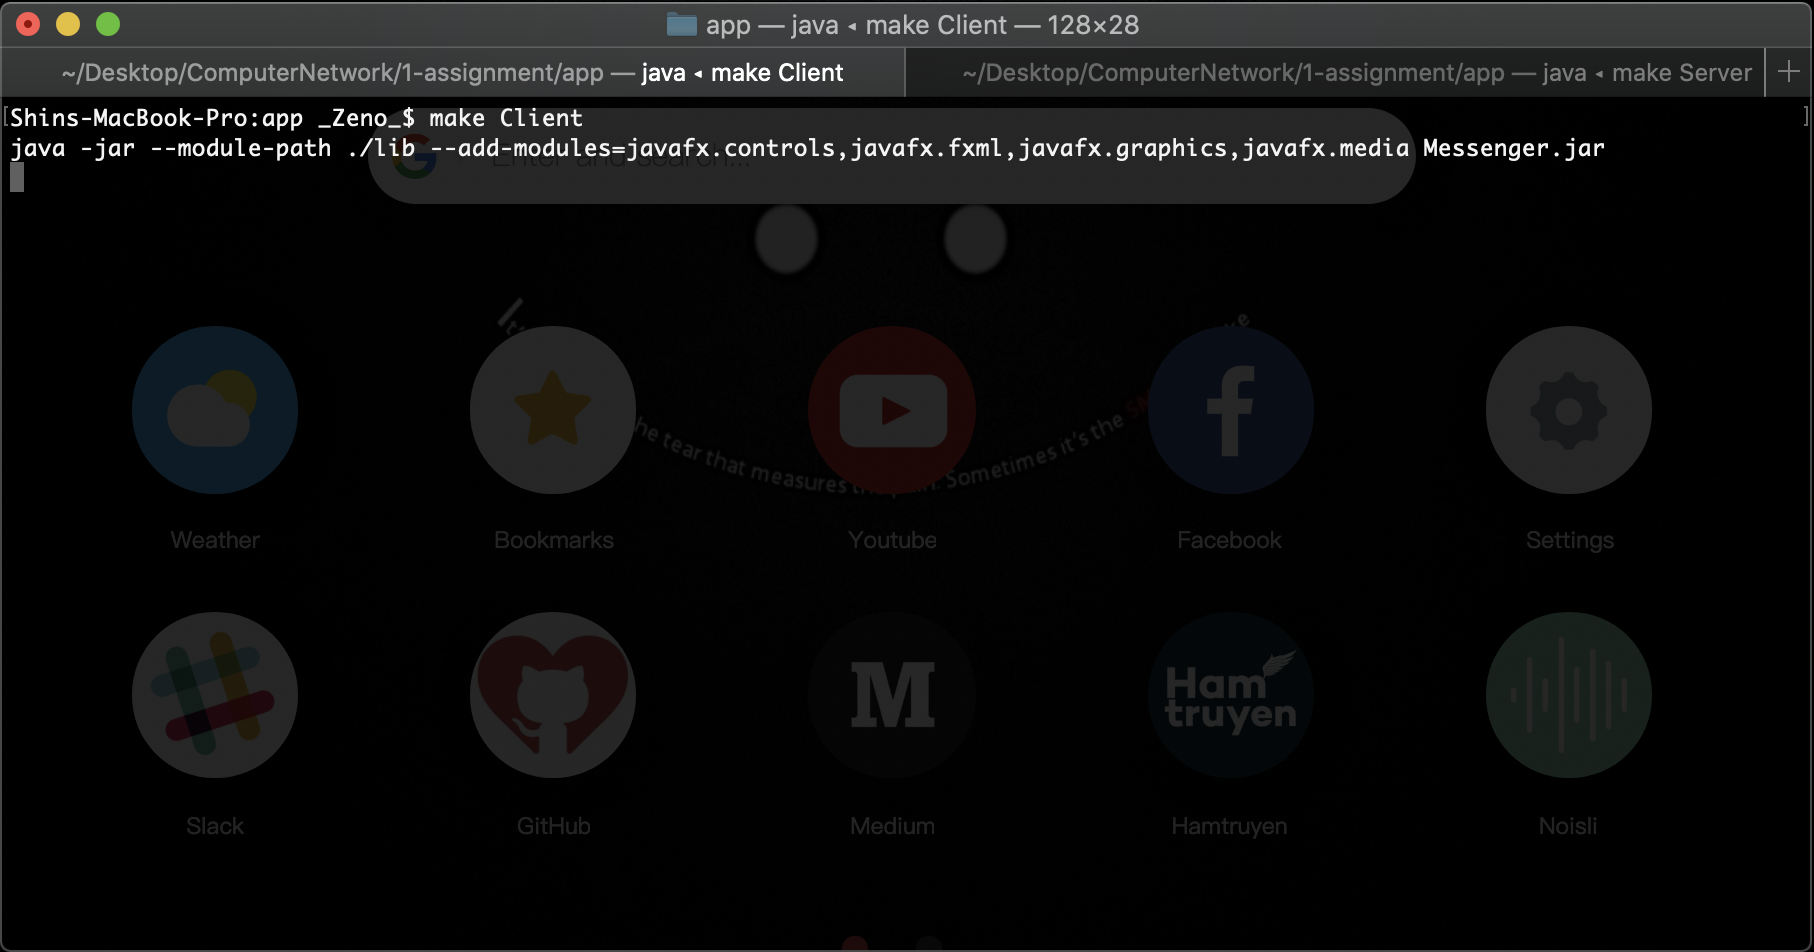
\includegraphics[width=9cm]{messenger-terminal} &
	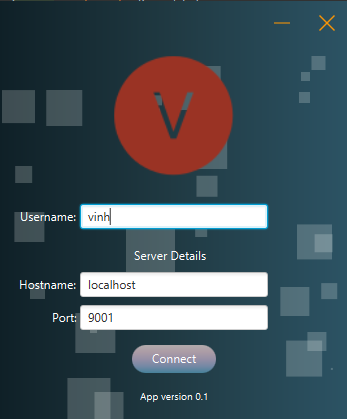
\includegraphics[width=4cm]{LogIn}
	\end{tabular}
	\caption{Cách mở messenger bằng terminal}
\end{figure}

Nếu muốn máy tính là một server, chạy dòng lệnh sau: {\tt make Server}

\begin{figure}[h!]
	\centering
	\begin{tabular}{c c}
	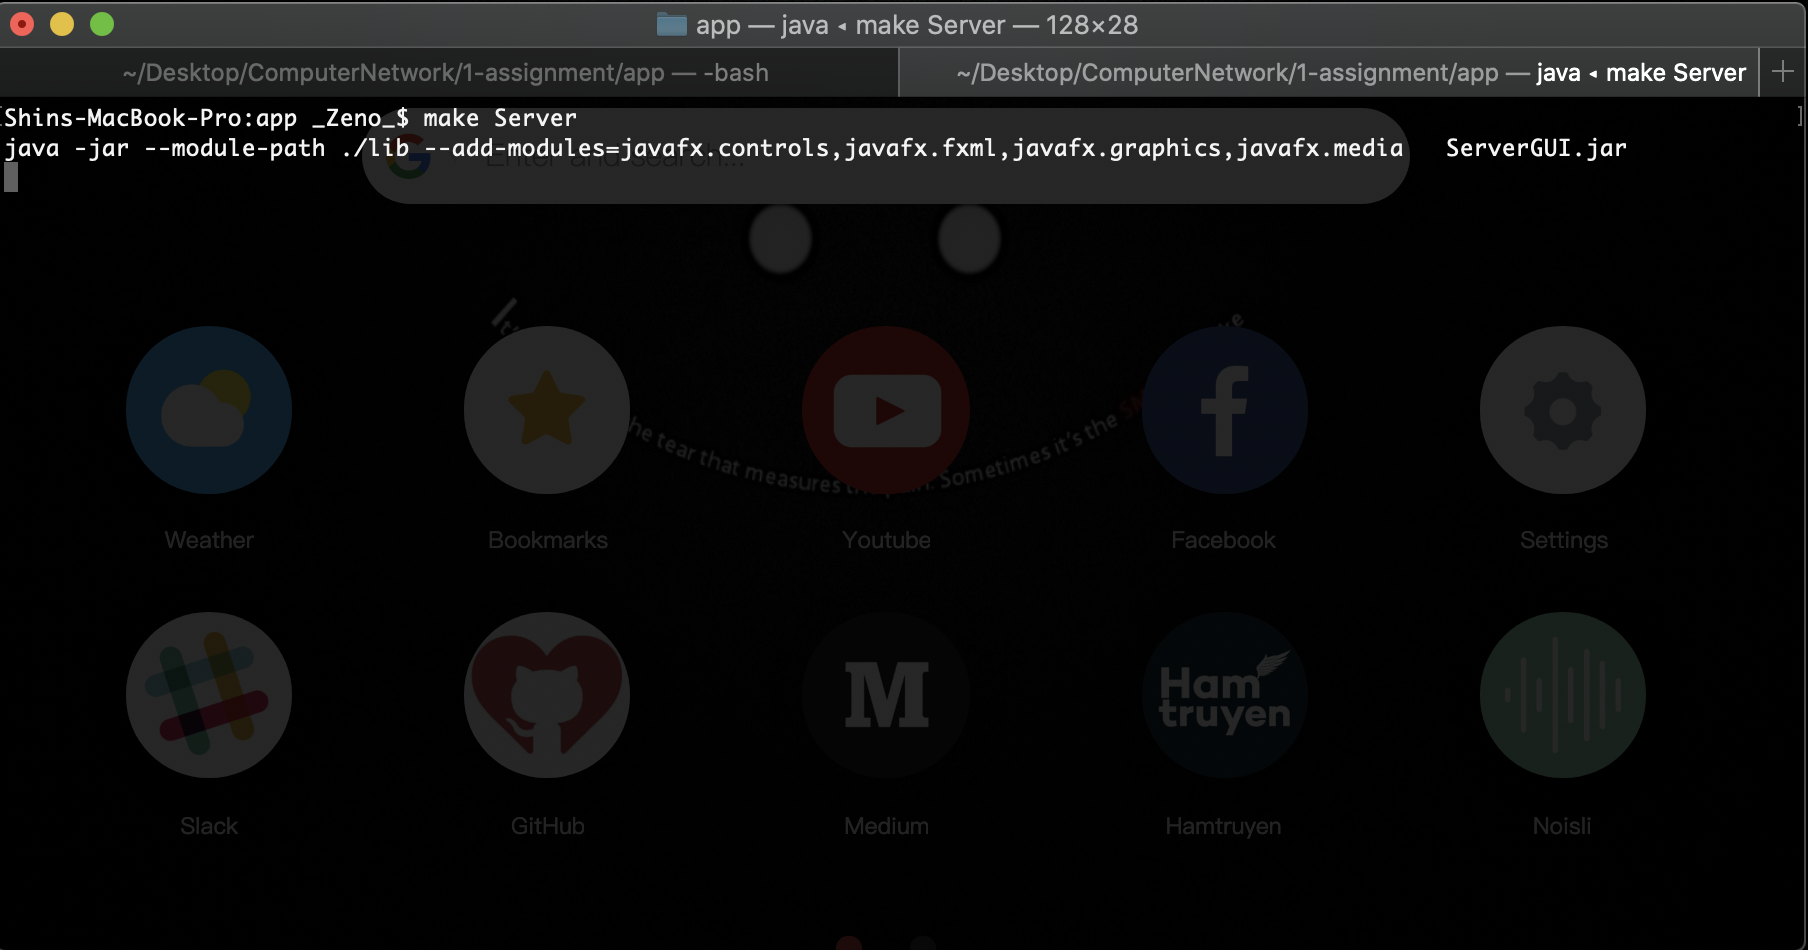
\includegraphics[width=9cm]{server-terminal} &
	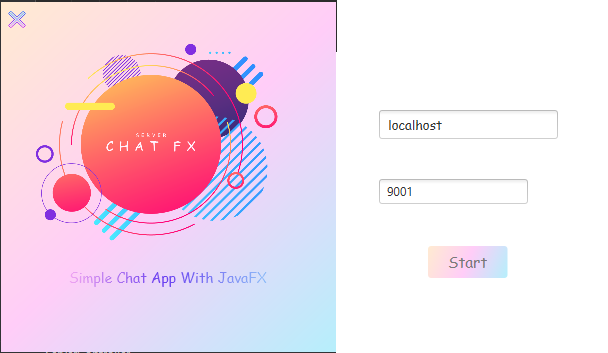
\includegraphics[width=5cm]{server_Launcher}
	
	\end{tabular}
	\caption{Cách mở server bằng terminal}
\end{figure}




\end{document}